\section{Introduction}

\begin{frame}{Problem of Interest}

    \textit{Investigating the distribution of flow velocity around a pillar during windy conditions to enhance personal comfort by determining the optimal position that reduces wind exposure.}

    \vspace{9pt}

    \begin{figure}

        \centering
        \includegraphics[height=0.45\textheight]{img/Grandate-Sergio.jpeg}
        \hfill
        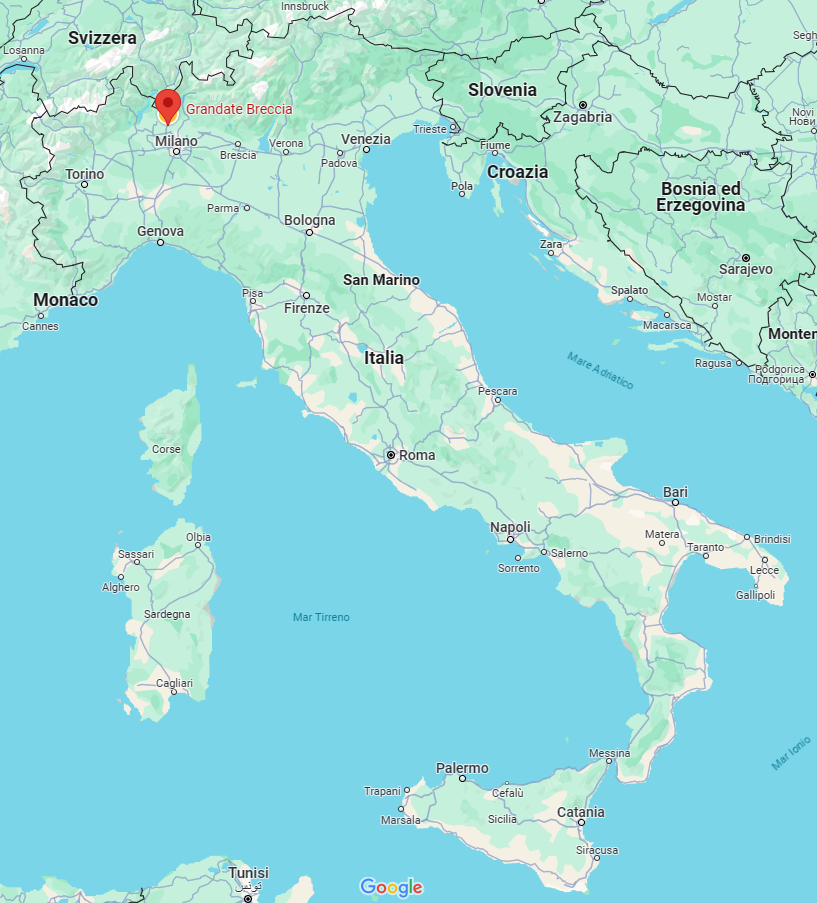
\includegraphics[height=0.45\textheight]{img/Italy-map.png}

        \caption{Grandate-Breccia train station\footnotemark[1], Como, Italy}

    \end{figure}

    \footnotetext[1]{Credit to S. Zerlottin for the picture (March 25, 2024)}

\end{frame}


\begin{frame}{Problem Statement}

    Here follow some questions that this study aims to answer:

    \begin{itemize}
        \item How does the wind speed affect the flow velocity distribution?
        \item How does the wind direction affect the flow velocity distribution?
        \item How does the geometry of the pillar affect the flow velocity distribution?
    \end{itemize}

    \vspace{9pt}

    In the end, \textbf{what's the optimal position to reduce wind exposure?}

\end{frame}
